\section{Experiments}
\label{sec:experiments}

This entire approach has been experimentally validated on a real system\footnote{Full video test available on \url{https://www.youtube.com/watch?v=oKMR_QCT7EE}}, composed by:

\begin{itemize}
	\item Asus Xtion Pro Live RGBD sensor.
	\item Turtlebot2 robot.
	\item Standard laptop computer. Hardware:
	\begin{itemize}
		\item CPU: Intel i5-4210U
		\item RAM: 8 GB DDR3L
		\item GPU: Nvidia 940M
	\end{itemize}
\end{itemize}

\begin{figure}[h]
	\centering
	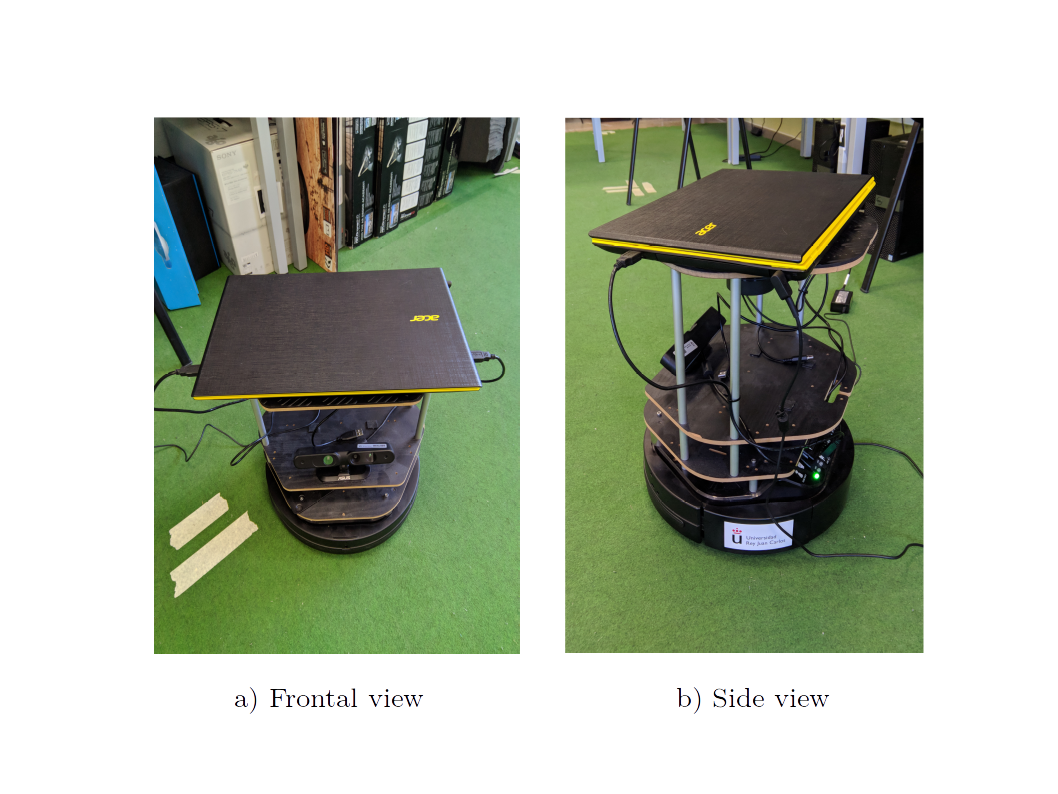
\includegraphics[width=4in]{images/exp_set}
	\caption{Experimental set where the system has been validated.}
	\label{fig:exp_set}
\end{figure}






The results have yielded a fine following system, which only follows to the indicated person, with a refresh rate of 10 movements per second (as the SSD CNN is the lightest possible model, as seen on Table \ref{tab:model_tests}. This helped substantially to minimize the time bottleneck). The tracking and reidentification process can be observed on the highest region of Fig. \ref{fig:exp_figures}. The following process can be observed on the lowest region of Fig. \ref{fig:exp_figures}.

\begin{figure}[h]
	\centering
	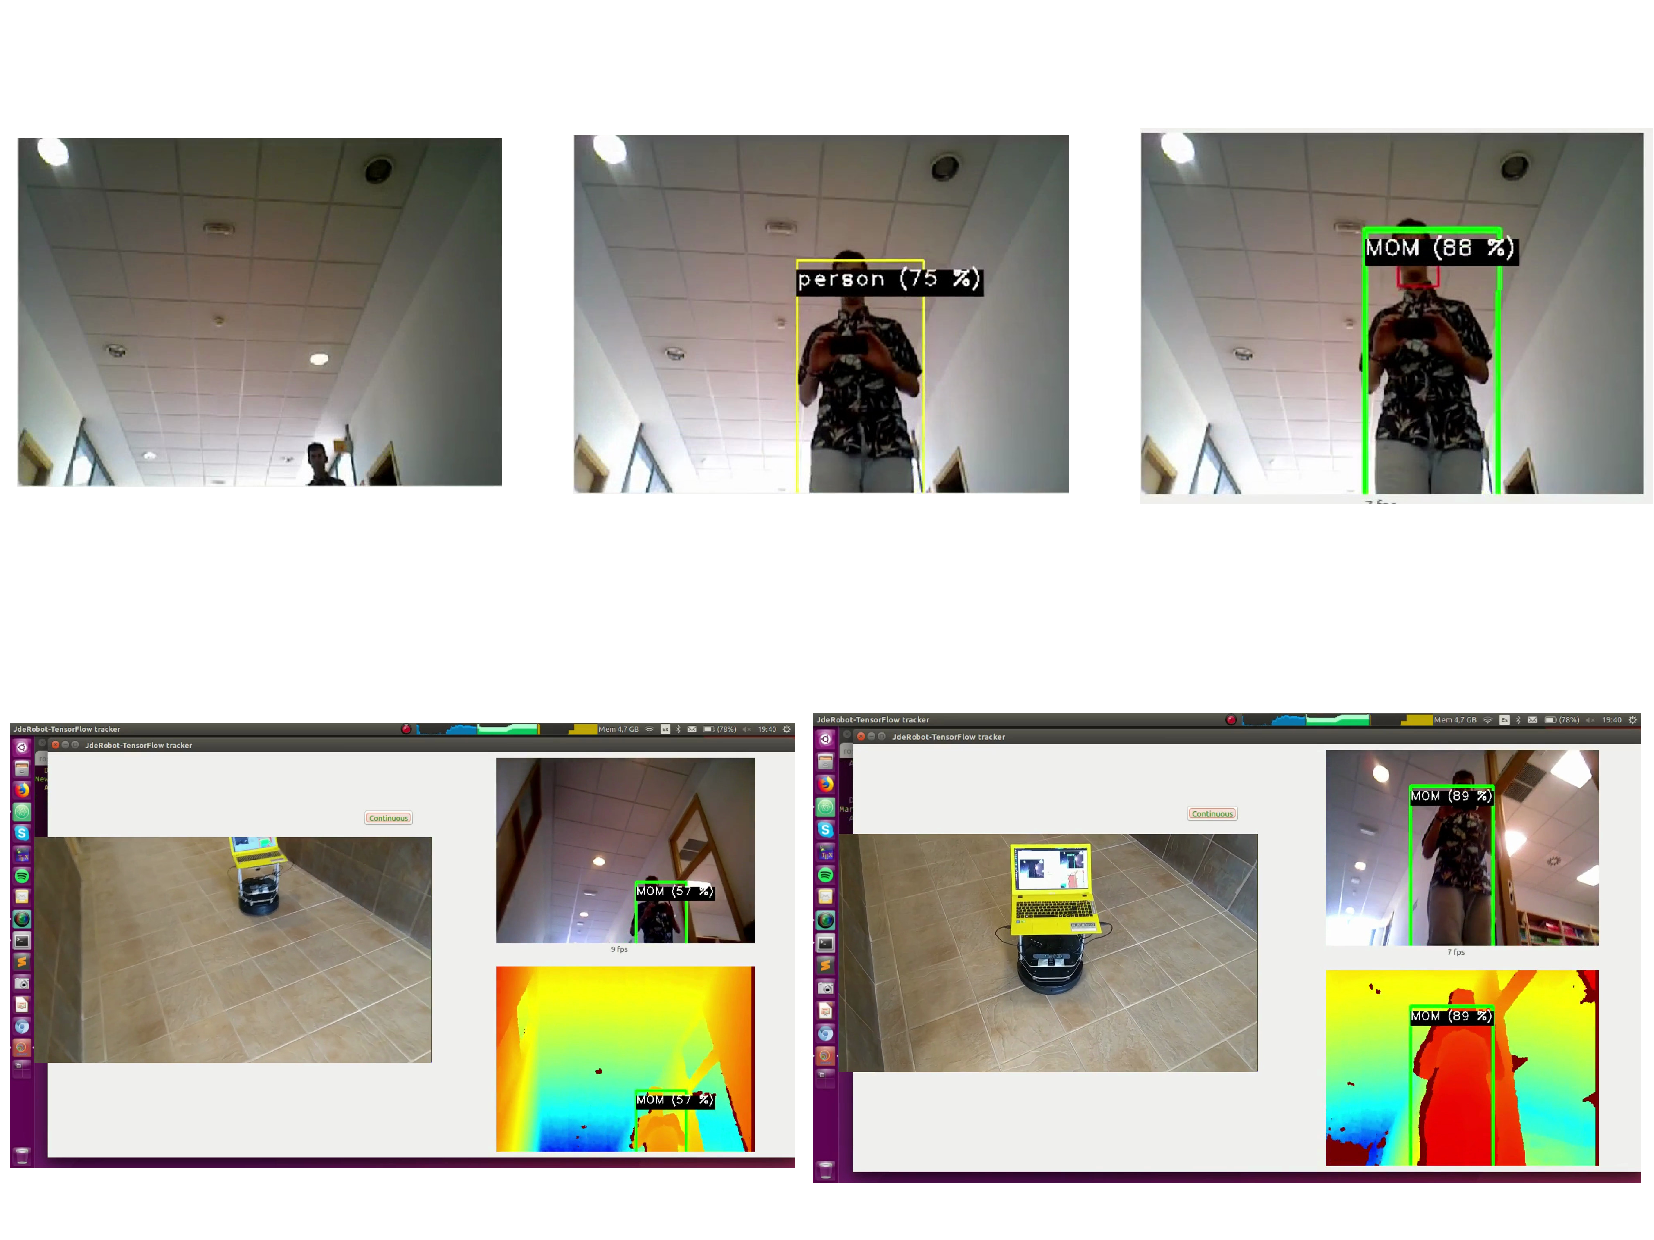
\includegraphics[width=2.5in]{images/exp_figures}
	\caption{Tracking and reidentification process for a person (up). Following process (down).}
	\label{fig:exp_figures}
\end{figure}